\chapter{Planning and Management}

This section will discuss planning approaches, time management, communications, budget, risks and division of tasks and responsibilities throughout the project.

\section{Agile: Lean Methodology}

Lean methodology was the agile approach chosen for delivering the product to the client. Lean guidelines are to eliminate anything not adding value to the product at the current moment in time. This is defined as creating more value for customers with fewer resources \cite{LeanEnterpriseInstituteLeanMethodology} used.

The team understood this as initially creating a very basic product to then add more complex features based upon client feedback. At every sprint, a fully functional system would be presented to the client. If the client was not satisfied, the team could easily make the necessary changes to revert to the previous functional system. 

The initial thought was to use a drone to collect data, with a plan to have a working product later in time. But, by using lean, this approach was changed to originally use a basic micro controller that could be improved in future sprints. This simplified the initial process, providing immediate, clear value to the client.

\subsection{Sprints}

The project consisted of three major technical sprints:

\begin{table}[H]
\centering
\begin{tabularx}{\textwidth}{|l|X|X|}
\hline
\textbf{Sprint} & \textbf{Description}                                                                                                                                                 & \textbf{Goal}                                  \\ \hline
1               & An investigation into oneM2M, deploying the chosen open source platform, and pass data though the platform from the Raspberry Pi HAT                                                     & Create a plug-in, and deploy an OM2M platform with single value sensors \\ \hline
2               & Investigation and experimentation with data federation between open source platforms to show how this will work with oneTRASNPORT. Interoperate with oneTRANSPORT & Demonstrating federation between OM2M, OpenMTC, and oneTRANSPORT by registering platforms as RemoteCSEs, and navigating into them.           \\ \hline
3               & Research and experimentation into data source showing upper limits of data being passed through platforms                                                                 & Supporting complex data streams, and create a video stream using oneM2M.               \\ \hline
\end{tabularx}
\caption{Technical Sprints}
\label{technical-sprints}
\end{table}

Lastly after Sprint 3, the team was focused on writing the final report as well as the presentation, poster and individual reflection.

\section{Time Management}

To manage time, Asana\footnote{The teams Asana page: \url{https://app.asana.com/0/84906964149735/list}} was used to create projects and deadlines and help structure time to ensure project tasks were completed on time. The functionality that Asana provided also helped manage and delegate tasks between ourselves.

\subsection{Gantt Chart}

The on-line tool Instagantt is a visualization platform that integrates Asana projects. This tool could be used to visualize the project as a Gantt Chart with deadlines and completed tasks inside a sprint. It provides an easy interface to manage the project, including marking a task as completed or extending the deadlines if a task was underestimated. 

\begin{figure}[H]
\centering
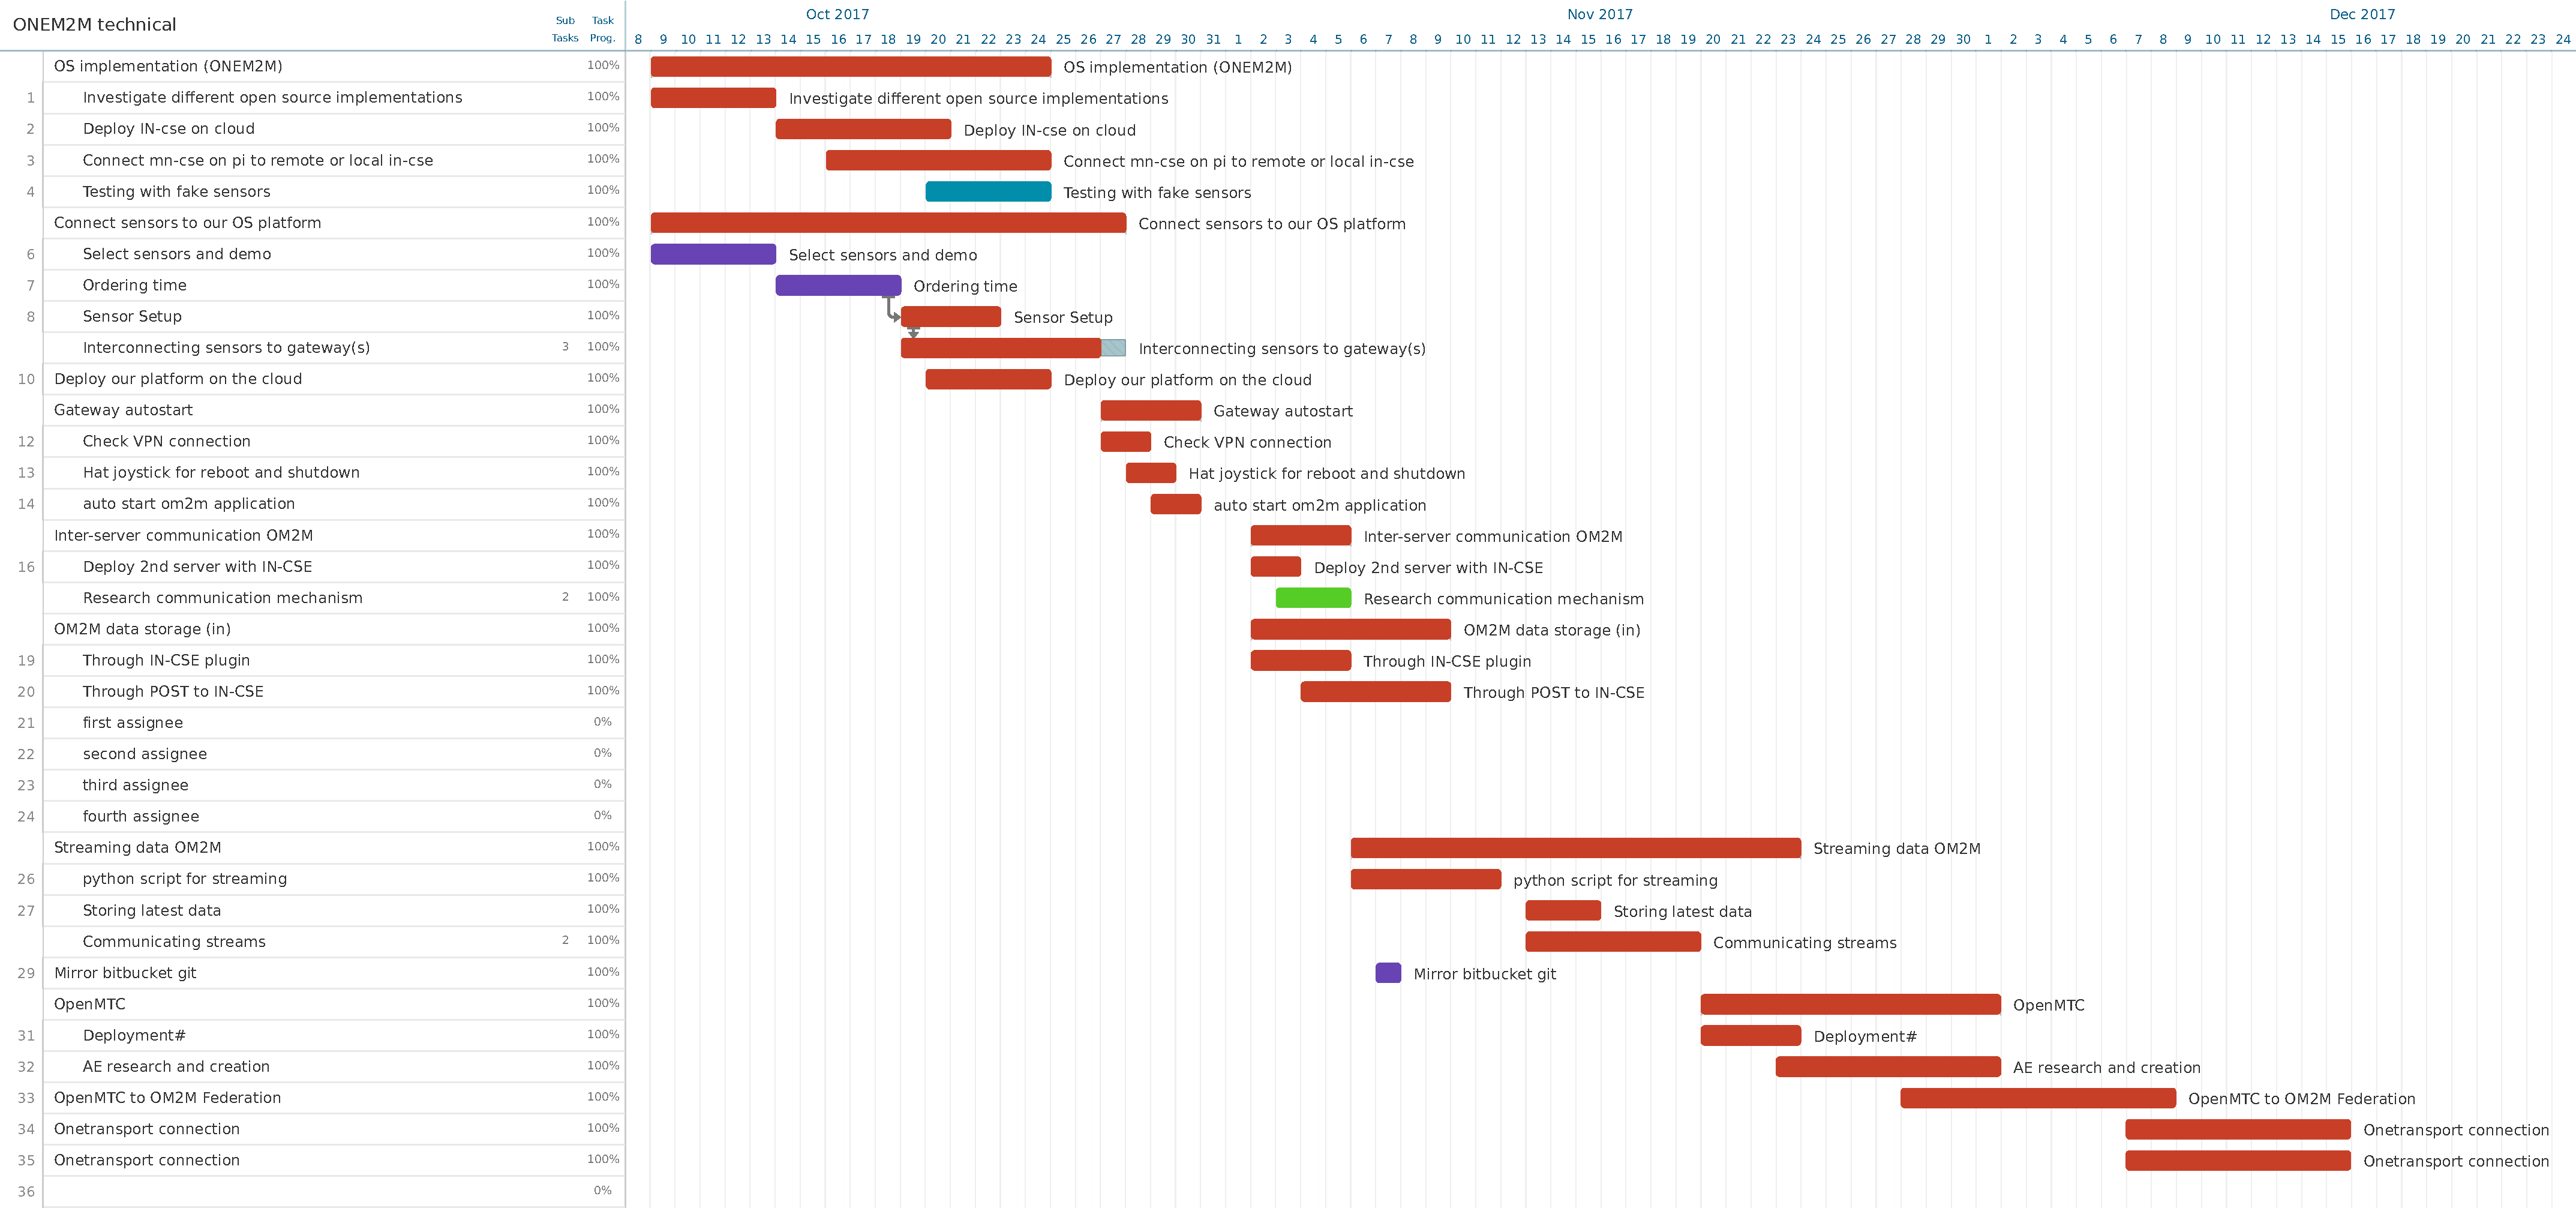
\includegraphics[width=\textwidth]{gatt}
\caption{Gantt Chart}
\label{fig:gantt-chart}
\end{figure}

The Gantt Chart above, is reproduced at a larger size in Appendix A.

The beginning of every sprint consisted of a team meeting where tasks and sub-tasks would be allocated for the current sprint and assigned to one or two team members. A preliminary deadline date for the task would be set based upon the estimated task difficulty (decided as a team). This method gave the team the ability to distribute their work load evenly between this project and other commitments (other modules).
 
\section{Communication}

During the initialisation of the group, the team's supervisor sent out a broadcast to the group to set up an initial meeting. During this meeting, it was established that a line of communication with the client, and between the group was necessary.

\subsection{Team Communication}

The tools used for communication between team members were Asana, Facebook Messenger and BitBucket. Facebook Messenger was used for daily remote communication and to update each other on progress or modifications to the project.

Additionally, there were numerous meetings in person as a group throughout the duration of the project. These meetings were both formally and informally arranged. This lead the team to work faster as each team member could aid each other in real time instead of having to wait for Facebook Messenger responses. 

BitBucket was used for the source code, where any team member could share and push updates. Automated builds were created using BitBucket, so whenever code that did not compile was pushed, it would not pass the verification checks and the team would be notified via email.

Overleaf was used for report writing, as it is an easy to use, on-line, collaborative \LaTeX\,environment. The downside is, that due to the nature of such system, it is harder, but not impossible to attribute work to individual team member, due to the absence of a \lstinline{git} log. To compensate for this, periodic backups were made using the download as zip functionality.

\subsection{Client Communication}

Throughout the whole process the client (InterDigital) was always up to date with the current progress. This ensured that the team remained on the right tracks. 

The tool used for communication with the client was mainly e-mail. Every week, on Friday, an e-mail was sent to the client updating them on progress. Included were certain elements of the project that needed feedback, such as the sensors, as well as any questions for them. Also, there was one onsite meeting with the client; this was the team's first interaction with the client, allowing for discussion of the specification of the project together to hash out all of the details. Finally, there were multiple Skype meetings with the client after every sprint in which the team would present, demo and discuss the work accomplished.  

\subsubsection{Online Tools}

\begin{itemize}
\item Facebook Messenger. Daily communication and updates on the project.
\item BitBucket. Used to share source code and work on tasks together.
\item Google Drive. For documentation.
\item LucidChart. For creating charts.
\item Asana. Used to manage and delegate tasks.
\item Overleaf. Used to create the final report in a synchronised and distributed manner.
\end{itemize}

\subsubsection{Meetings}

\begin{itemize}
\item First with supervisor, where notes were taken, and then with each other.
\item Group Supervisor. To update about progress, discus concerns (if anyone had any) and GS would advise if needed. Notes were also taken at these meetings.
\item Client. One in person meeting, numerous Skype meetings. Notes were also taken at these meetings.
\item Group. Almost daily meet-ups at the university computer labs, therefore everyone was up to date and progress was being made day by day.
\end{itemize}

Additionally, every Friday, emails were sent to inform the client about the team's progress.

\subsection{Client Feedback}

As well as updating the client on project progress and asking questions to clear up any confusion about the project, client feedback was requested. Throughout the project this feedback was taken into consideration to help shape the project in such a way that the client would be satisfied with the result. This lead to significant changes and shifts so that the client would be truly satisfied with the result.

The significant changes include, but are not limited to:

\begin{itemize}
  \item \textbf{Scrapping the Dashboard}\\Originally, the team was going to produce a HTML5 dashboard to federate, report, and automate the sensors. However, after talking to the client, it was felt that this was not necessary. The client already had a system for gathering and visualising the data using a Graphite database and a Grafana fronted.
  \item \textbf{Scrapping the Drones}\\As stated previously the initial idea was to use drones to collect data, however a Raspberry Pi was decided to be used instead. The main task of this project was to show federation using the oneM2M standard and this could be done much more simply by using a Raspberry Pi with basic sensors.
\end{itemize}

\section{Budget}

Without a concrete budget, InterDigital decided to provide the team with equipment and services. Table \ref{resource-payment-information} are purchases throughout the project with their corresponding description and price. 

\begin{table}[H]
\centering
\begin{tabularx}{\textwidth}{| X | l | l |}
\hline
\textbf{Resource} & \textbf{Cost} & \textbf{Paid By}
\\ \hline
2x \textbf{Raspberry Pi 3Bs} for development (\url{https://thepihut.com/products/raspberry-pi-3-model-b}) & 2x£32 & InterDigital 
\\ \hline
2x \textbf{Raspberry Pi SenseHATs} to provide sensor data (\url{https://amazon.co.uk/dp/B014T2IHQ8/}) & 2x£29.27 & InterDigital 
\\ \hline
2x \textbf{8GB microSD cards} to store the Operating System & 0 & N/A
\\ \hline
2x \textbf{microUSB cables} to power the Raspberry Pis & 0 & N/A
\\ \hline
1x \textbf{Raspberry Pi Camera Module 2}, to experiment with still image capture and video streaming & £22.50 & InterDigital 
\\ \hline
1x \textbf{sensivision.co domain name}, a centralised domain name was needed to point to & £12 & Us
\\ \hline
2x \textbf{Digital Ocean Droplet} @ £10/mth to host the oneM2M and OpenMTC server & 2x£10/mth & Us
\\ \hline
1x \textbf{LetsEncrypt} free HTTPS certificate for sensivision.co & Free & N/A
\\ \hline
\end{tabularx}
\caption{Resource Payment Information}
\label{resource-payment-information}
\end{table}

Some of the costs were paid out of pocket due to time constraints. It was felt that it would be easier to do so.

\section{Risk}

At the start of the project potential risks that may occur throughout the project were identified. And mitigations to reduce the impact (probability $\times$ severity) were proposed. These are listed in the following table: 

\begin{table}[H]
\begin{adjustwidth}{-1.5cm}{-1.5cm}
\centering
\caption{Risk Assessment}
\label{risk-assessment}
\addvbuffer[0em 1em]{\begin{tabularx}{\textwidth+3cm}{| m{8cm} | l | X | m{6cm} |}
\hline
\textbf{Risk Description} & \textbf{Prob.} & \textbf{Sev.} & \textbf{Mitigation} \\
\hline
\textbf{Cloud server access}

The client (InterDigital) agreed to provide a cloud server on Azure. This allows them to have direct access to the server after the project has finished. Before the start of the project that cloud was accessed, but server administration would be necessary (such as opening ports). The team did not have administrator access to the cloud hosting dashboard to configure the instance. If communications with the client took too long this could prevent project progress. &    High & High & It was agreed with InterDigial that if using their Azure account would block the project progress, the team would use a cloud service provider (Digital Ocean), over which the team would have admin dashboard control. At the end of the project InterDigital would be provided documentation on how to reproduce the server-side environment. \\
\hline
\textbf{Access to oneTRANSPORT Server} 

The aim of this project is too see whether and how two separate implementations of the oneM2M standard could communicate with each other. To do this, Eclipse OM2M was used for the implementation. Afterwards the aim was to connect to the oneTRANSPORT server. The client may not grant full access to their system and the progress of this task may be slow. & High & High & If access to oneTRASNPORT is limited or indirect, federation would be shown with another open source platform implementation using the oneM2M standard (OpenMTC). The documentation would be provided to the client to allow them to reproduce the federation within their environment and hardware. \\
\hline
\textbf{Team member absence}

Be it injury, sickness, or just missing, a missing team member has the potential to delay the project. But fortunately given the team size, even if it is more probable, it will be easier to compensate due to team size.& Med. & Low & Using pair programming, therefore there is never work that is not understood by just one team member.\\
\hline
\textbf{Poor Team Dynamic}

The team not getting along and communications breaking down between individual members, or the team as a whole. This could lead to a minor set-back, or the team completely fracturing and falling apart. & Low & High & Constant communication. Talks with supervisor to ensure everything is okay. If there were problems they were expressed during supervisor meetings. \\
\hline
\textbf{Loss of Data}

Loosing important code and / or documents due to poor planning and decision making by the team resulting in a significant setback, ultimately delaying the project.& Low & High & Usage of remote repositories such as Bitbucket / Github in order have non-local copy of project development. \\
\hline
\end{tabularx}}
Probability and Severity are abbreviated.
\end{adjustwidth}
\end{table}

\section{Task Distribution}

Project Manager: Dennis Parchkov

At the beginning of the project the team met together to introduce ourselves. After thoroughly getting to know each other and every member's respective skills, the tasks were able to be distributed accordingly shown in table \ref{task-distribution}.

\begin{table}[H]
\centering
\begin{tabularx}{\textwidth}{|l|l|X|}
\hline
\textbf{Member}              & \textbf{Expertise} & \textbf{Tasks}           				\\ 
\hline
Adib Pournazari     & Python           & OpenMTC Scripting. 				\\ 
\hline
Altay Adademir      & Web              & Deployment, Web Development.              				\\
\hline
Dennis Parchkov     & Python           & oneM2M Research, Team Communication, Project Management.                				\\
\hline
Edmond Ipindamitan  & Java             & oneM2M Research, Sensivision Plug-in.			\\ 
\hline
Matthew Consterdine & Raspberry Pi    & Automation, Raspberry Pi Python Scripts, Combining Java and Python, Unit and Integration testing, Formatting and Proofing.	\\ \hline
\end{tabularx}
\caption{Task Distribution}
\label{task-distribution}
\end{table}

All the team contributed to the report, with each member starting work on the sections they felt most familiar with. Once a foundation was laid, different team members helped to improve and revise the report, ensuring that it flowed into one cohesive whole.

Because of how the team collaborated on the report, attributing any one section to any one member is impossible. Each member helped work on every section of the report, writing new content, revising existing content, and removing that which was no longer needed.

\clearpage
